\chapter{Related Work}

There are a wide variety of methods that are used in the field of emotion recognition using facial expressions. However, a large number of those methods are implemented using a similar process. Shown in Figure ~\ref{fig:process}, initially the image is captured and processed. Thereafter the face is detected and features are extracted. Then a machine learning technique is trained to do the classification of the emotions. 

\begin{figure}[ht]
  \centering
  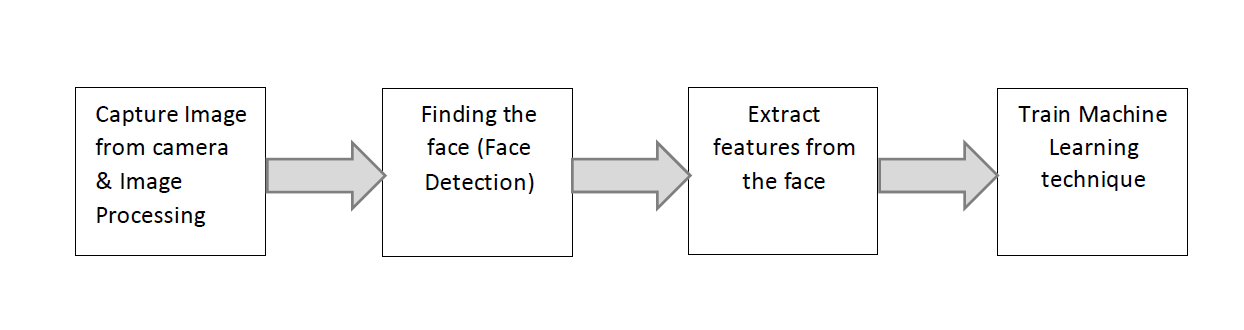
\includegraphics[scale=0.4]{4}
  \caption{The four stages for facial expression recognition}
  \label{fig:process}
\end{figure}
The related work looks at all four stages in the implementation process and different methods used by other researchers. The rest of this chapter is organised as follows: Section 2.1 describes the process of obtaining the image from the camera and image processing; Section 2.2 explains how face detection functions; Section 2.3 explains the feature extraction process; Section 2.4 the training of the machine learning technique and Section 2.5 outlines the results achived by other researchers.
%---------------------------------------------------------------
\section{Capture Image from the Camera and Image Processing}
An image is taken from the camera and image processing tools are used to help normalize and standardize the input image.
\begin{itemize}

\item Goyal and Mittal, achieved the desired resolution and colour for their images by adjusting the brightness and contrast of the image\cite{1}.

\item Reddy and Srinivas, scaled and cropped their images to \textit{(150X120)}, and ensured that the location of the eyes stayed the same in each image. The image was processed further, using an average combination of all the input image histograms. This process is called histogram equalization, see Figure~\ref{fig:hist eq}, and helps in decreasing variation in an image. Histogram equalization is a technique for stretching out the intensity range of an image to enhance the contrast of the image\cite{2}.

\begin{figure}[ht]
  \centering
  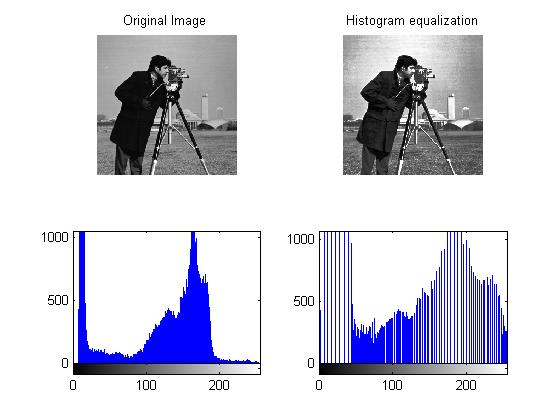
\includegraphics[scale=0.4]{5}
  \caption{Histogram Equalization}
  \label{fig:hist eq}
\end{figure}

\item Boubenna and Lee, scaled their images to \textit{(100X100)} pixels\cite{3}.

\end{itemize}
%---------------------------------------------------------------
\section{Face Detection - Finding the Face  }

Finding the location of the face helps identify the region that contains all the features required to continue with facial expression recognition. The rest of the image is not important for this purpose.
\begin{itemize}
\item Reddy and Srinivas applied a fixed oval shaped mask over the image to extract the face region\cite{2}. The images they used only contained faces, making it easier to apply the masks.

\begin{figure}[ht]
  \centering
  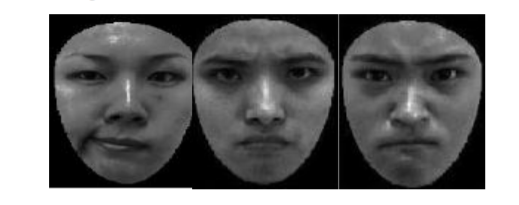
\includegraphics[scale=0.4]{6}
  \caption{Preprocessed Image with Oval Masks}
\end{figure}

\item Boubenna and Lee used the Viola and Jones algorithm to detect the location of the face in an image\cite{viola}. This algorithm uses Haar-like features to help find the facial features, such as the eyes, nose and mouth. The Ada Boost algorithm is used to reduce the number of features, if there are too many. They used the canny edge detection operator to detect the edges of the face\cite{3}.
\end{itemize}

%---------------------------------------------------------------

\section{Feature Extraction - Extract the Features from the Face }
Once the face has been detected, it is important to identify which features will be used for feature extraction. Either the full-face, or individual features from the face can be used as part of the feature set. These individual features can be the eyes, nose, mouth and eyebrows. The feature extraction algorithm can be applied based on its compatibility with the features chosen. 
\begin{itemize}
\item\ Goyal and Mittal extracted the nose, mouth and eyes using the Viola and Jones Haar classifier\cite{1}.

\item Reddy and Srinivas considered the entire face for the feature extraction not just the eyes, mouth and nose individually . First, they used Gabor filters to generate a bank of filters at 5 spatially varying frequencies and 8 orientations. The filtered outputs were then concatenated. Principle Component Analysis(PCA) was used to reduce dimensionality. PCA is a statistical technique that reduces the dimensions of feature vectors. The high dimensionality of feature vectors can cause over-fitting during classification. The PCA algorithm generates the eigenfaces for each image of dimension\textit{(NXN)}. From this their system generated the eigenvector of dimension \textit{(N2)} for each image. The vectors that relay the distribution of the face images the best are selected. These vectors are used to define the subspace(“face space”) of the face images\cite{2}. The face image subspace represents a lower dimentional space\textit{(N2)} of the original image with dimentions\textit{(NXN)}.

\item Boubenna and Lee used Pyramid Histogram of Oriented Gradients(PHOG) to extract features. PHOG represents an image by its local shape and the spatial layout. The local shape of an image is represented by a histogram of edge orientations within an image sub-region, which are divided into K bins. The spatial layout is represented by tiling the image into regions at different levels. Each image is divided into a sequence of increasingly finer spatial grids by repeatedly doubling the number of divisions in each axis direction\cite{phog}. The parameters of PHOG were set as follows: 3 for number of levels, 360 degrees for the number of dimentions and 16 for the number of bins. To decrease the number of features, a Genetic Algorithm(GA) was used, which resembles natural selection to find optimal features\cite{3}.
\end{itemize}

%---------------------------------------------------------------

\section{Training the machine learning technique}
The training of the machine learning technique based on supervised learning whereby the machine learning technique is given labelled images (Happy, Sad, Anger, Disgust, Surprise, Fear and Neutral) and is required to learn them. Once the machine learning technique has completed its training, it can then be fed unlabelled images, and the result would be a prediction of which label best suits the given image. 
\begin{itemize}
\item Goyal and Mittal used an Artificial Neural Network, with one hidden layer. The neural network architecture has three layers: input, hidden and output layers. Figure ~\ref{fig:nn} provides a visual layout of the architecture of an individual neuron and a ANN with multiple layers. Feed-forward ANNs allows the signal to travel in one direction from the input layer to the output layer. Recurrent networks contain feedback connections, where the signal moves in both directions. To get accurate results from the ANN, the weights can be set explicitly using prior knowledge, or the ANN can be trained to help find the optimal weights\cite{1, ann}.
\begin{figure}[ht]
  \centering
  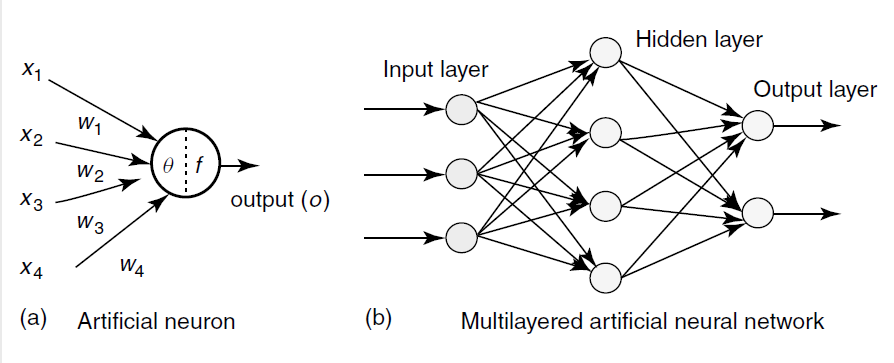
\includegraphics[scale=0.4]{8}
  \caption{Architecture of an artificial neuron and a multilayered neural network }
  \label{fig:nn}
\end{figure}
\item Reddy and Srinivas, used an Artificial Neural Network, with two hidden layers\cite{2}. 
\item Boubenna and Lee, used Linear Discriminants Analysis(LDA) and K Nearest Neighbours(KNN). LDA finds the maximum distances within classes, to obtain maximum class separation. LDA only uses up to second order moments, such as the covariance and mean, of the class distribution. KNN classifies unlabelled samples according to the training samples. KNN finds the nearest K in the labelled samples and set them to the closest group, for the unlabelled samples. One distance measure is required, and \cite{3} used the cosine distance measure.
\end{itemize}
%---------------------------------------------------------------
\section{Results}
The results from the three studies are as follows, with \cite{3} having the best overall results for their facial expression recognition system.
\begin{itemize}
\item Goyal and Mittal achieved an 80\% classification accuracy, using a confusion matrix and a regression plot to verify the results\cite{1}.
\item Reddy and Srinivas achieved an 85.7\% classification accuracy using the JAFFE database\cite{2}.
\item Boubenna and Lee achieved a 99.33\% accuracy, using the Radboud Faces Database(RaFD)\cite{3}.
\end{itemize}


